
\appendix
\section{Proof of Lemma \ref{lemma:kernel}}
\begin{proof}
We first prove (1) and (2). Since the Gaussian kernel \(K\) is \(C^\infty\) on \(\mathbb R^d\), so is its rescaling \(K_h\), and hence so is the convolution
\[
\tilde K_h = K_h * K_h.
\]
Therefore \(\tilde K_h\in C^\infty(\mathbb T^d)\). Moreover,
\[
\nabla \tilde K_h = (\nabla K_h)*K_h = K_h * (\nabla K_h).
\]
Since \(K_h,\nabla K_h\) are smooth and periodic on the compact domain \(\mathbb T^d\), it follows that
\[
\|\nabla \tilde K_h\|_{L^\infty(\mathbb T^d)}<\infty.
\]
Hence \(\nabla \tilde K_h\in L^\infty(\mathbb T^d)\), proving (2). By the mean value theorem on the torus, for any \(\bx,\by\in\mathbb T^d\),
\[
|\tilde K_h(\bx)-\tilde K_h(\by)|
\le \|\nabla \tilde K_h\|_{L^\infty(\mathbb T^d)}\,|\bx-\by|,
\]
so \(\tilde K_h\) is globally Lipschitz. This proves (1).

We now prove (3). Let \(v\in H^1(\mathbb T^d)\). Since differentiation commutes with convolution on \(\mathbb T^d\),
\[
\nabla(\tilde K_h * v)= \tilde K_h * \nabla v.
\]
We use Fourier series on \(\mathbb T^d\). Writing
\[
v(\bx)=\sum_{k\in\mathbb Z^d}\hat v_k e^{2\pi i k\cdot \bx},
\]
we have
\[
\widehat{K_h*v}_k=\widehat{K_h}(k)\hat v_k,
\qquad
\widehat{\tilde K_h*v}_k=\widehat{\tilde K_h}(k)\hat v_k.
\]
Since \(\tilde K_h=K_h*K_h\),
\[
\widehat{\tilde K_h}(k)=\widehat{K_h}(k)^2.
\]
For the Gaussian kernel, \(\widehat{K_h}(k)\to 1\) as \(h\to0\) for each fixed \(k\in\mathbb Z^d\), hence
\[
\widehat{\tilde K_h}(k)\to 1
\qquad\text{for each }k\in\mathbb Z^d.
\]
Therefore,
\[
\widehat{\nabla v-\nabla(\tilde K_h*v)}(k)
=
(2\pi i k)\bigl(1-\widehat{\tilde K_h}(k)\bigr)\hat v_k.
\]
By Parseval's identity,
\[
\|\nabla v-\nabla(\tilde K_h*v)\|_{L^2(\mathbb T^d)}^2
=
\sum_{k\in\mathbb Z^d}
(2\pi)^2 |k|^2\,|1-\widehat{\tilde K_h}(k)|^2\,|\hat v_k|^2.
\]
Now for every \(k\), \(0\le \widehat{\tilde K_h}(k)\le 1\), so
\[
|1-\widehat{\tilde K_h}(k)|^2\le 1.
\]
Since \(v\in H^1(\mathbb T^d)\), the sequence
\[
(2\pi)^2 |k|^2 |\hat v_k|^2
\]
is summable. Thus, by dominated convergence,
\[
\|\nabla v-\nabla(\tilde K_h*v)\|_{L^2(\mathbb T^d)}\to 0
\qquad\text{as }h\to0.
\]

It remains to prove the quantitative estimate for \(v\in H^2(\mathbb T^d)\). For the Gaussian kernel one has
\[
\widehat{K_h}(k)=e^{-\pi^2 h^2 |k|^2},
\qquad
\widehat{\tilde K_h}(k)=e^{-2\pi^2 h^2 |k|^2}.
\]
Using the elementary inequality \(1-e^{-t}\le t\) for \(t\ge0\), we obtain
\[
|1-\widehat{\tilde K_h}(k)|
=
1-e^{-2\pi^2 h^2 |k|^2}
\le 2\pi^2 h^2 |k|^2.
\]
Hence
\[
\begin{aligned}
\|\nabla v-\nabla(\tilde K_h*v)\|_{L^2(\mathbb T^d)}^2
&=
\sum_{k\in\mathbb Z^d}
(2\pi)^2 |k|^2\,|1-\widehat{\tilde K_h}(k)|^2\,|\hat v_k|^2 \\
&\le
C h^2 \sum_{k\in\mathbb Z^d} |k|^4 |\hat v_k|^2.
\end{aligned}
\]
Since
\[
\sum_{k\in\mathbb Z^d} |k|^4 |\hat v_k|^2
\sim \|D^2v\|_{L^2(\mathbb T^d)}^2,
\]
it follows that
\[
\|\nabla v-\nabla(\tilde K_h*v)\|_{L^2(\mathbb T^d)}
\le Ch\|D^2v\|_{L^2(\mathbb T^d)},
\]
where \(C>0\) is independent of \(h\). This completes the proof.
\end{proof}
\section{Addition result for one dimensional linear benchmark}

\begin{figure}[htbp]
    \centering
    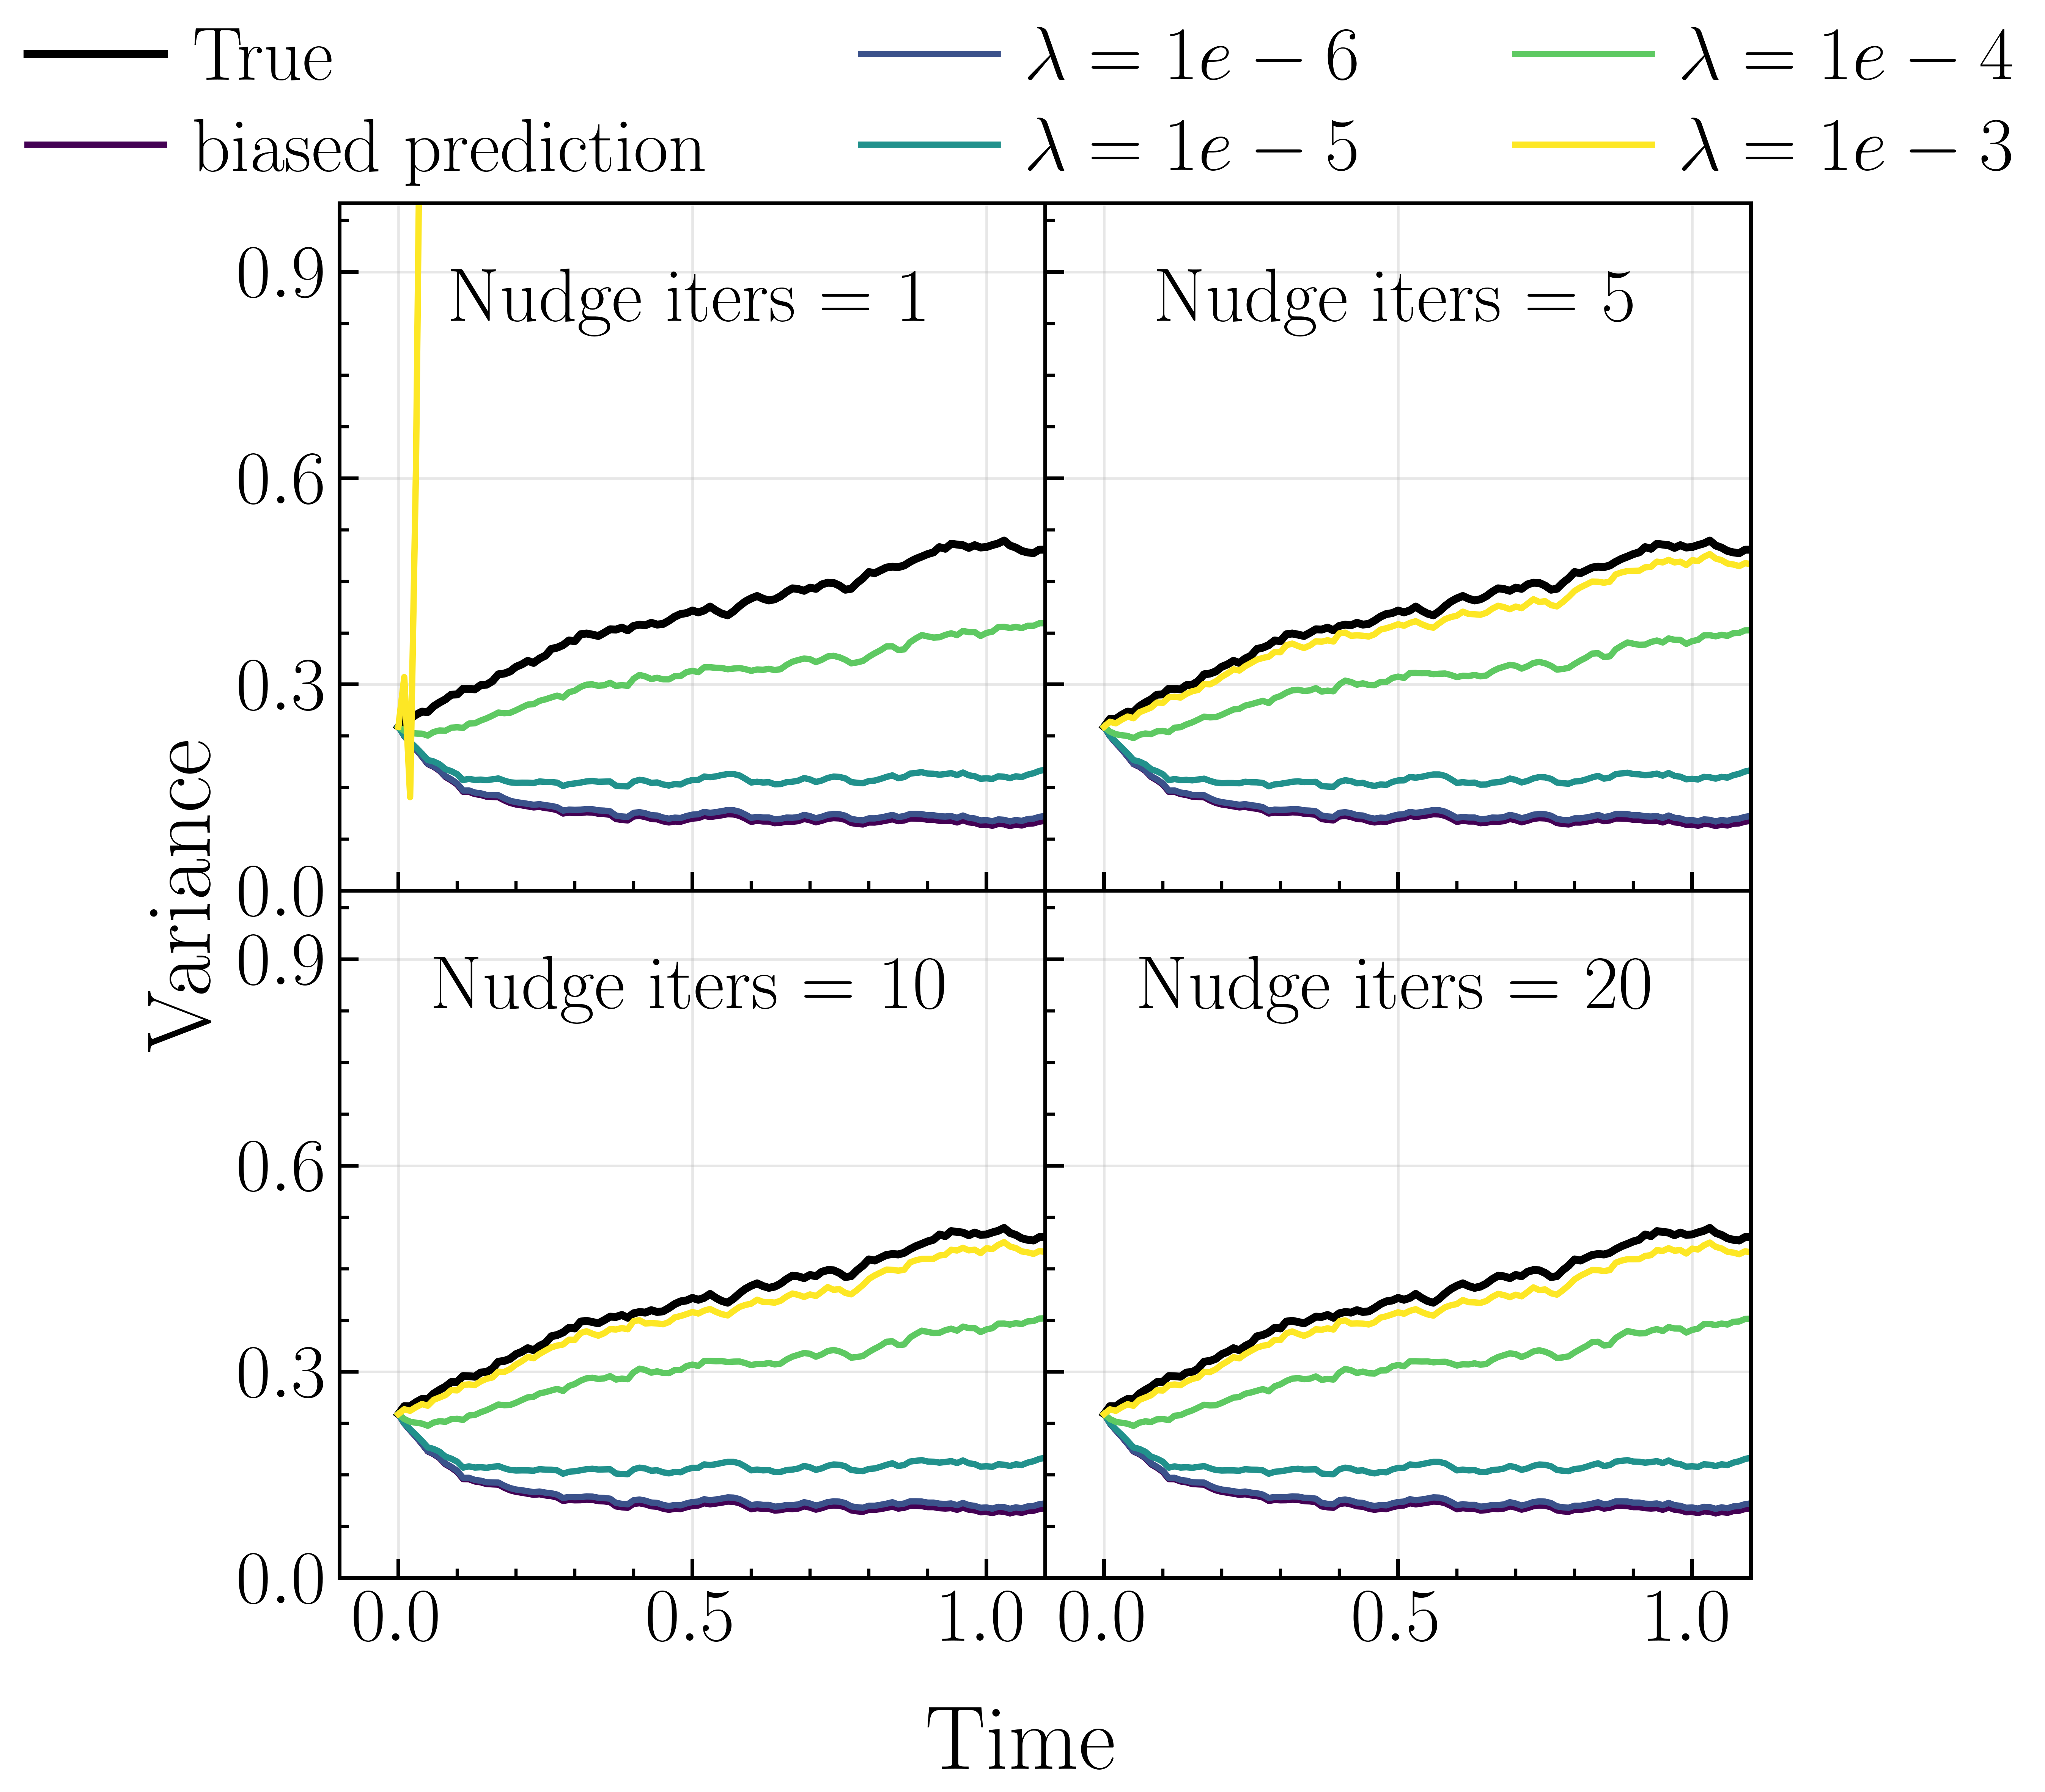
\includegraphics[width=0.8\textwidth]{../figure/1d_case_a_2.png}
    \caption{\textbf{Variance dynamics in the one-dimensional linear benchmark ($a=2$).} We compare the reference system, the biased forecast model, and assimilated (nudged) trajectories with $\lambda\in\{10^{-6},10^{-5},10^{-4},10^{-3}\}$. Increasing $\lambda$ generally improves tracking accuracy, but excessively large nudging may reduce numerical stability.}
    \label{fig:simple_linear_case_a_2}
\end{figure}

\begin{figure}[htbp]
    \centering
    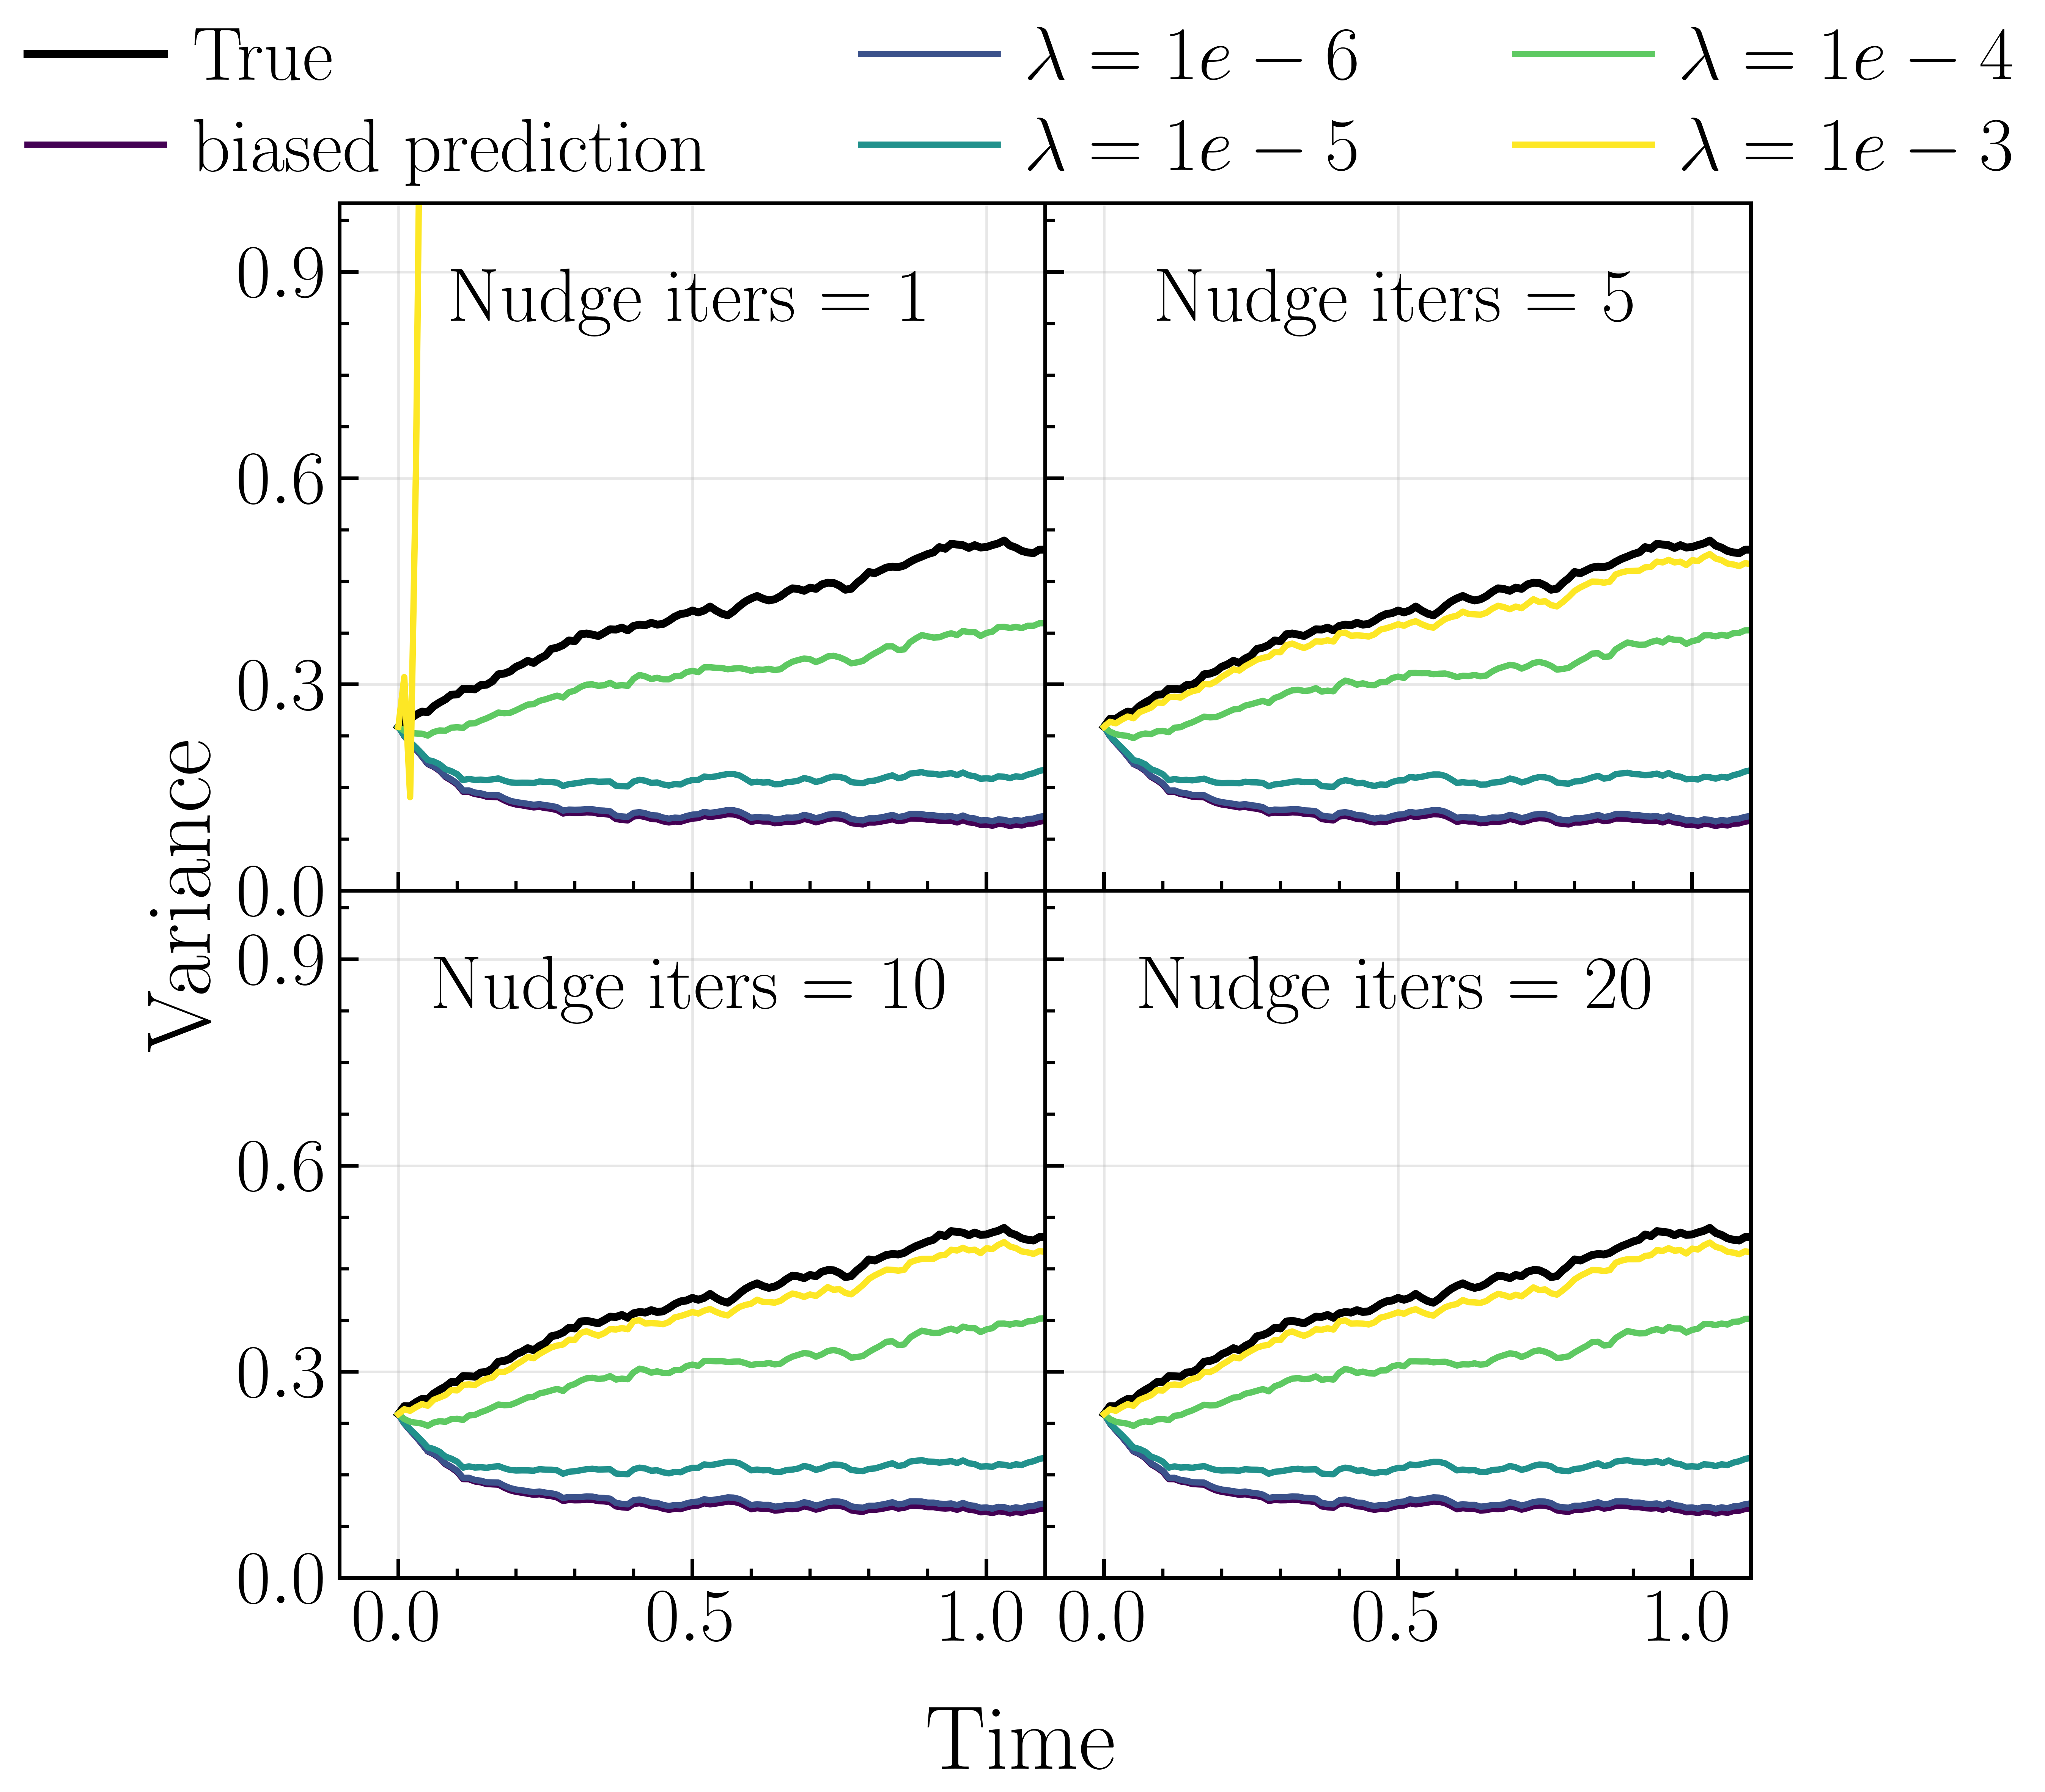
\includegraphics[width=0.8\textwidth]{../figure/1d_case_a_5.png}
    \caption{\textbf{Variance dynamics in the one-dimensional linear benchmark ($a=5$).} We compare the reference system, the biased forecast model, and assimilated (nudged) trajectories with $\lambda\in\{10^{-6},10^{-5},10^{-4},10^{-3}\}$. Increasing $\lambda$ generally improves tracking accuracy, but excessively large nudging may reduce numerical stability.}
    \label{fig:simple_linear_case_a_5}
\end{figure}
